\section{Evaluation}

We evaluate FourShadow using $128\times128\times K$ SGEMM kernels, where
$K\in\{128,256,512,1024\}$. Each experiment changes one architectural
parameter while holding the remaining configuration fixed. Speedups are
calculated from total kernel cycles against the corresponding baseline
configuration.

\subsection{Scaling Across the SIMT Hierarchy}\label{sec:eval_hierarchy}

\subsubsection{Threads/Warp}
Fig.~\ref{fig:threads_sweep} compares TCU SGEMM with scalar FP32 execution
at the same thread count. Packing more low-precision elements raises
speedup from 3.55--6.44$\times$ for TF32 to 9.53--27.46$\times$ for FP8.
Most notably, we find that the 16-thread configuration is consistently the strongest and reaches
27.46$\times$, while increasing to 32 threads (the established default warp-size in all modern GPU architectures) does not improve performance
further. This shows that Tensor Core scaling is non-monotonic with warp width
and depends significantly on tile geometry and pipeline utilization.

\begin{figure} [h]
    \centering
    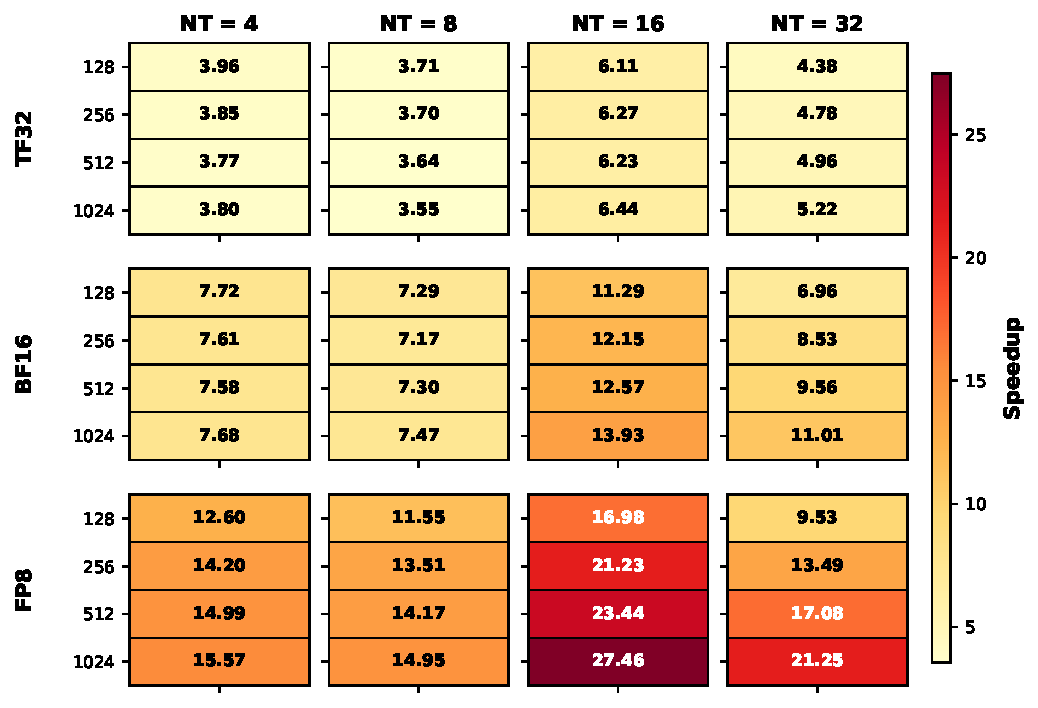
\includegraphics[width=0.9\linewidth]
    {hpca2027-latex-template/fig/sgemm_speedup_heatmap_v3_gaplabel.pdf}
    \caption{SGEMM speedup over scalar FP32 execution across
    threads/warp and input precisions.}
    \label{fig:threads_sweep}
\end{figure}

\subsubsection{Warps/Warpgroup (Issue Width)}
Fig.~\ref{fig:iw_sweep} normalizes each configuration against an issue
width of one. An issue width of two provides 1.21--1.48$\times$ speedup,
while four reaches up to 1.84$\times$. Increasing to eight only peaks at 2.02$\times$, with the 8- and 16-thread designs largely saturating after
four and the 32-thread design even regresses. This proves that wider issue provides diminishing returns once operand delivery and
non-TCU execution become the dominant costs.
\begin{figure}
    \centering
    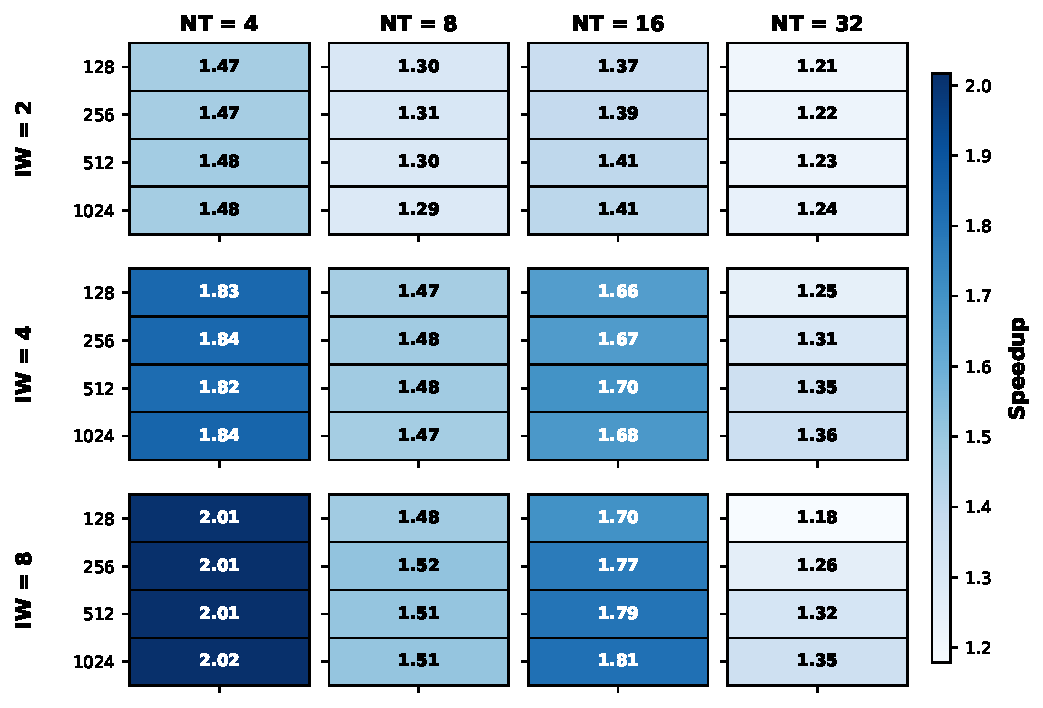
\includegraphics[width=0.9\linewidth]
    {hpca2027-latex-template/fig/iw_speedup_heatmap_blue_v1.pdf}
    \caption{BF16 WGMMA speedup over an issue width of one across
    threads/warp and issue-width configurations.}
    \label{fig:iw_sweep}
\end{figure}


\subsubsection{Cores/Socket}
Fig.~\ref{fig:cores_sweep} shows that the 4-thread configuration scales
nearly linearly, reaching 7.23$\times$ with eight cores. Note-worthily, core scaling falls as
the warp width grows, with the 32-thread configuration reaching only
3.27--5.10$\times$, although larger $K$ values partially recover its efficiency.
Core-level scaling therefore heavily depends on preserving enough independent
output tiles, since wider per-core tiles reduce grid-level concurrency
and increase the impact of workload partitioning and tail effects.
\begin{figure}
    \centering
    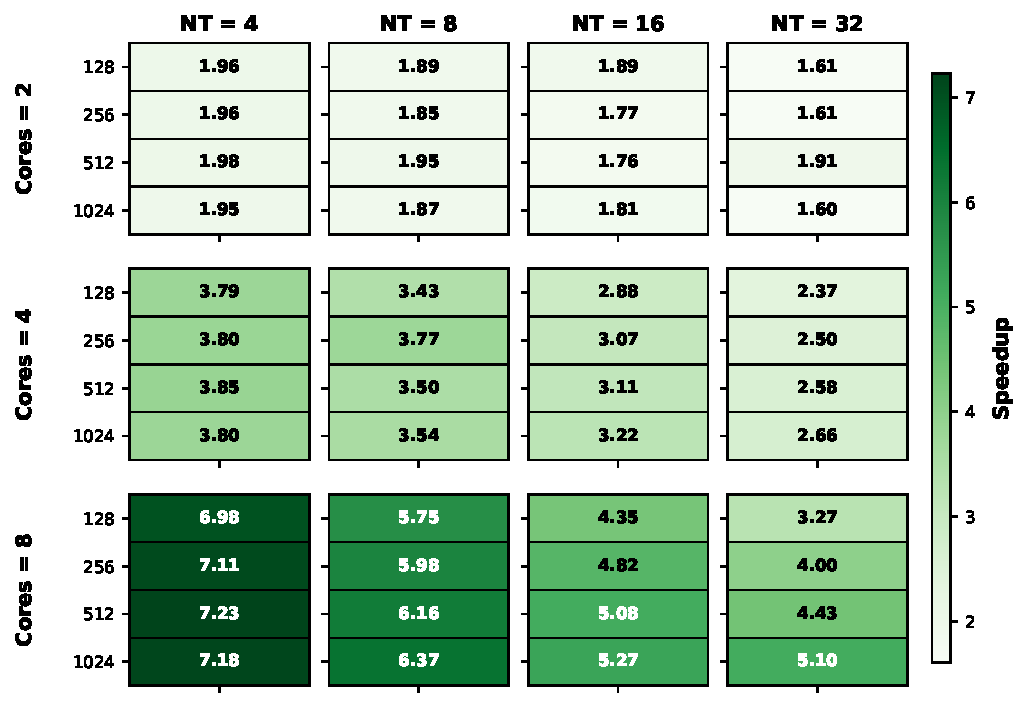
\includegraphics[width=0.9\linewidth]
    {hpca2027-latex-template/fig/cores_speedup_heatmap_green_v1.pdf}
    \caption{FP16 WGMMA speedup over a single core as the number of
    cores/socket is increased.}
    \label{fig:cores_sweep}
\end{figure}

\subsubsection{Roofline Model Performance Analysis}
Fig.~\ref{fig:roofline} shows that WMMA raises arithmetic intensity from
0.25 to 3.61 FLOP/byte and throughput from 2.65 to 23.21 FLOP/cycle.
Sparse WMMA further reaches 33.49 FLOP/cycle. On the other hand, while WGMMA has the highest achieved operational intensities at 5.82 and 7.11 FLOP/byte, it only reaches 2.31 and
5.85 FLOP/cycle for dense and sparse execution respectively. This indicates that Tensor Core designs, especially with sparsity enabled are able to move fairly memory-bound kernels into the compute bound region. WGMMA seems to be improving arithmetic intensity specifically from it's larger operating tiles and shared-memory reuse, making it particularly suitable for modern ML systems inference or LLM Decode workloads that are significantly more memory-bound than compute-bound. 
\begin{figure}
    \centering
    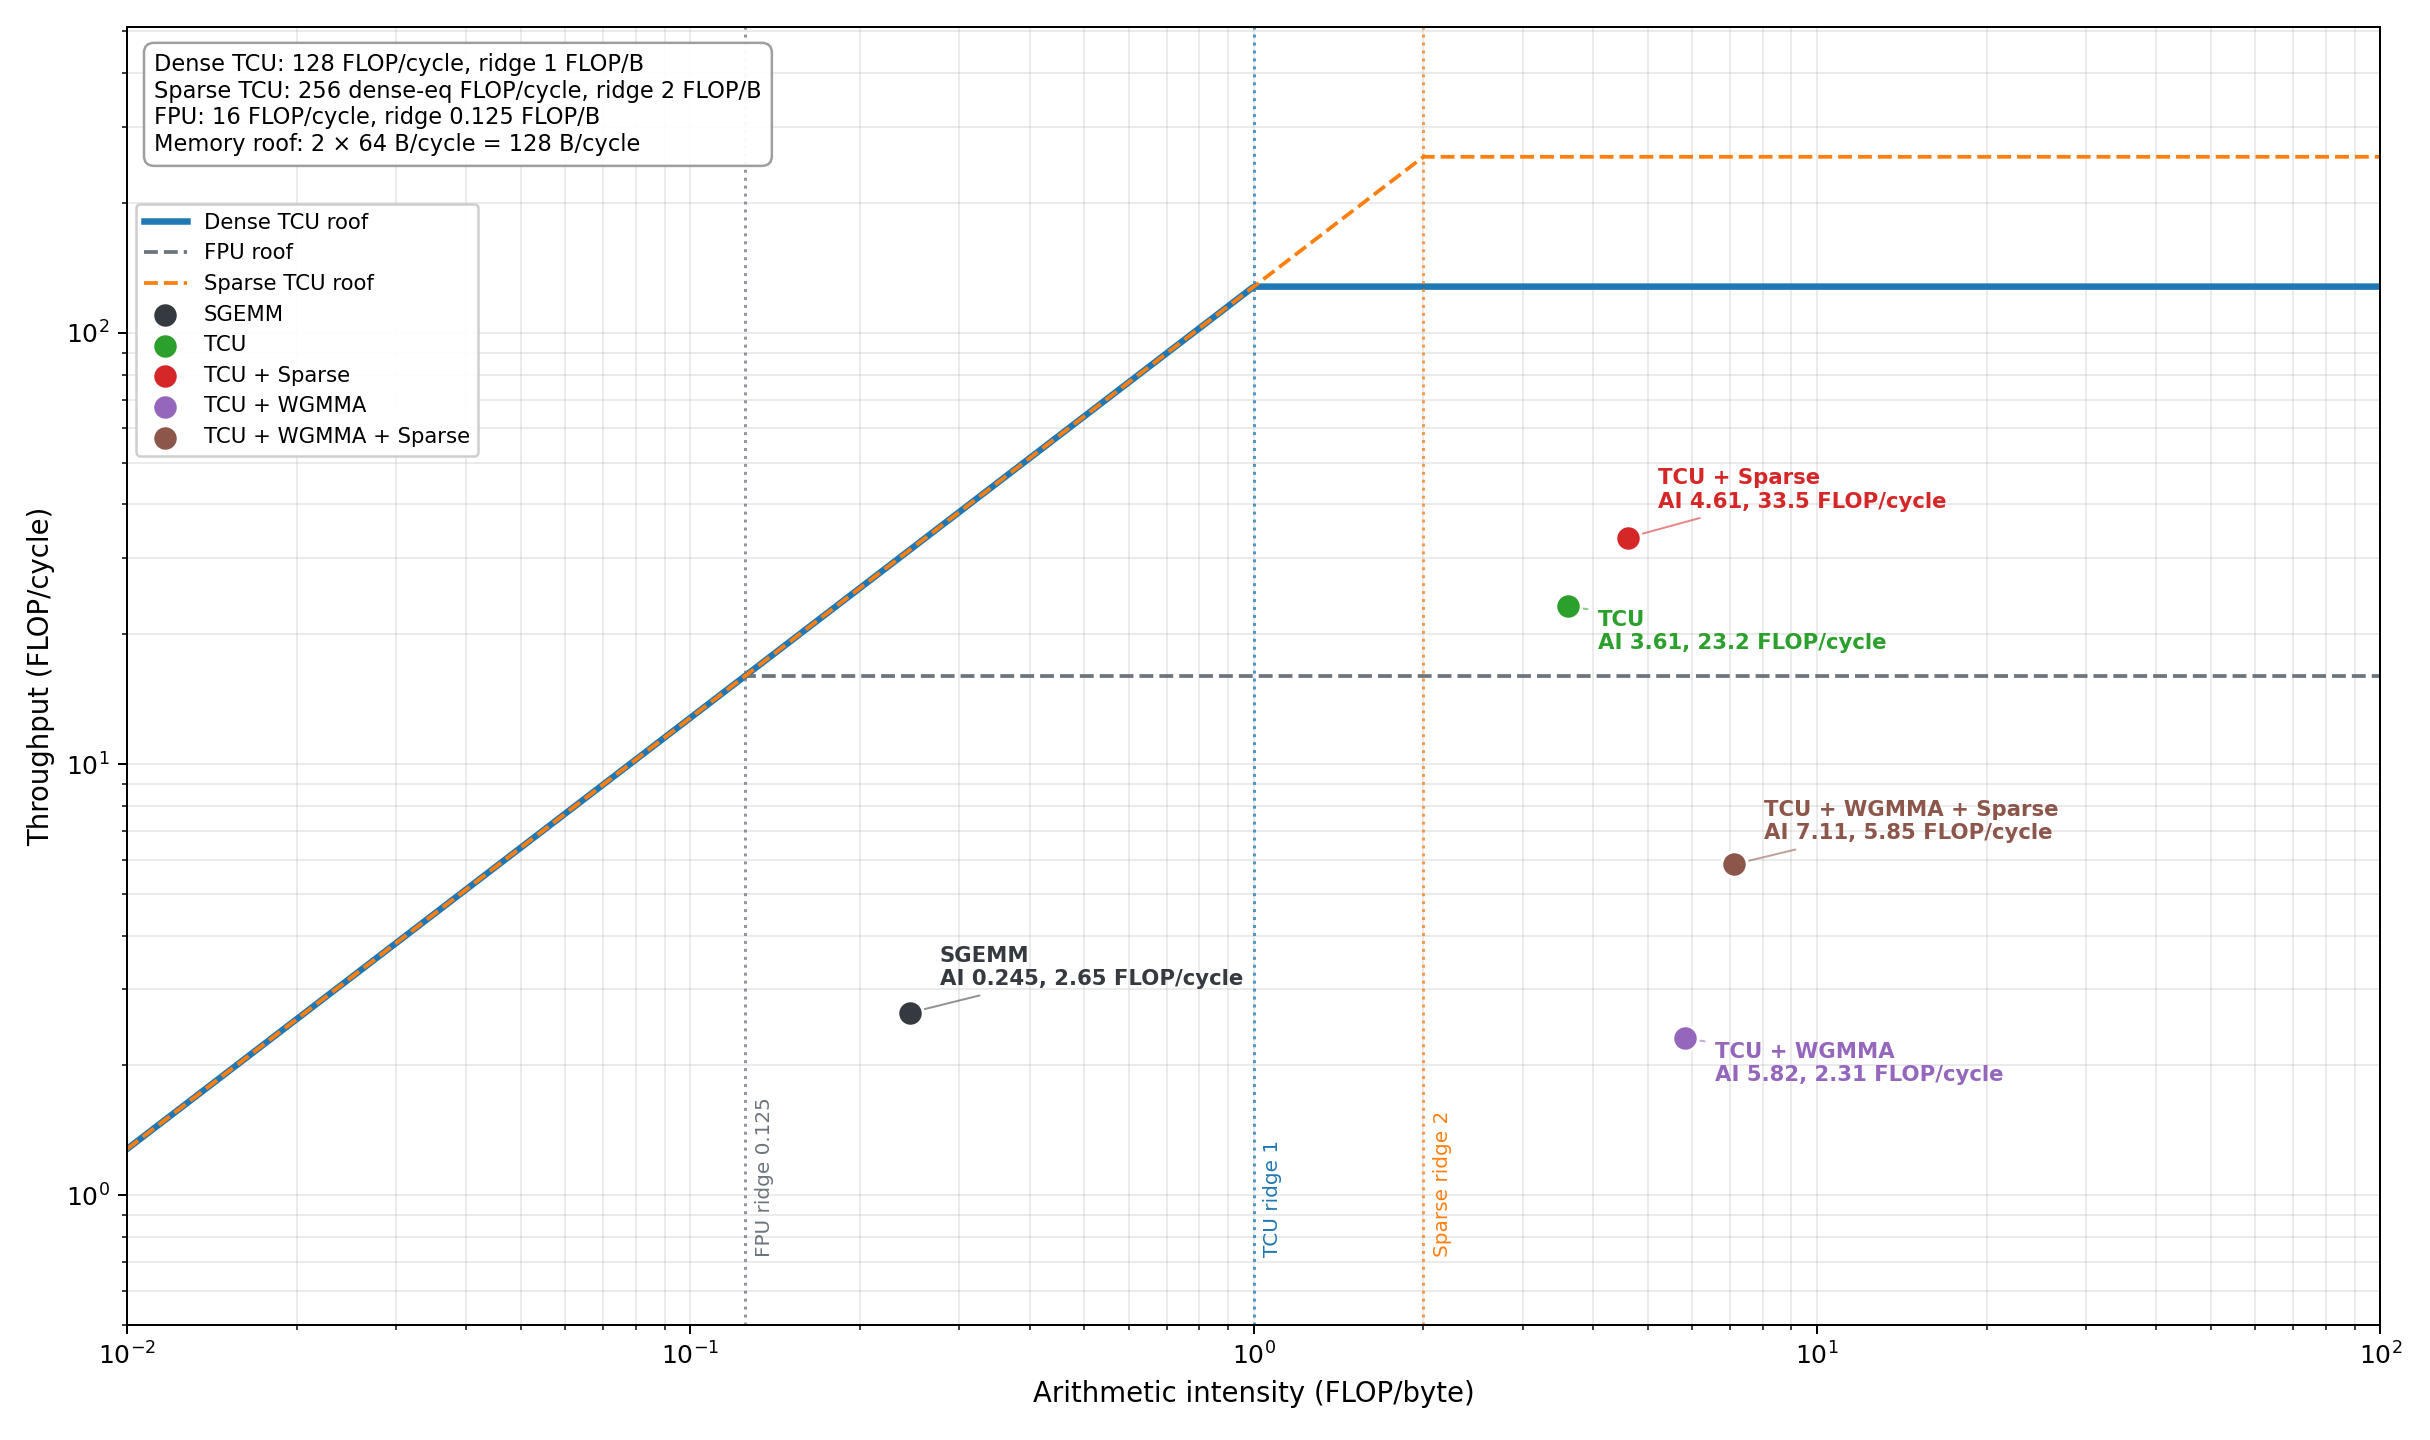
\includegraphics[width=\linewidth]
    {hpca2027-latex-template/fig/roofline_128_compare.png}
    \caption{Roofline comparison of scalar, WMMA, WGMMA, and
    2:4 sparse execution for a $128^3$ SGEMM kernel.}
    \label{fig:roofline}
\end{figure}

\subsection{Warp-Group Tensor Core Design Space Exploration}\label{sec:eval_wgmma}

\subsubsection{Number of Accumulator Registers (NRC) Scaling}
As shown in Fig.~\ref{fig:nrc_sweep}, increasing NRC from 8 to 16 reduces
cycles by 30--32\% in both RS and SS modes. Extending SS to NRC${}=32$
reduces cycles by approximately 49\% over NRC${}=8$. SS is only 1--4\%
faster than RS at the same NRC, so its main advantage is mostly enabling the
largest accumulator tile size possible. However, the gains remain sublinear because memory,
control, and outer $K$-loop work do not shrink with accumulator capacity.
\begin{figure}
    \centering
    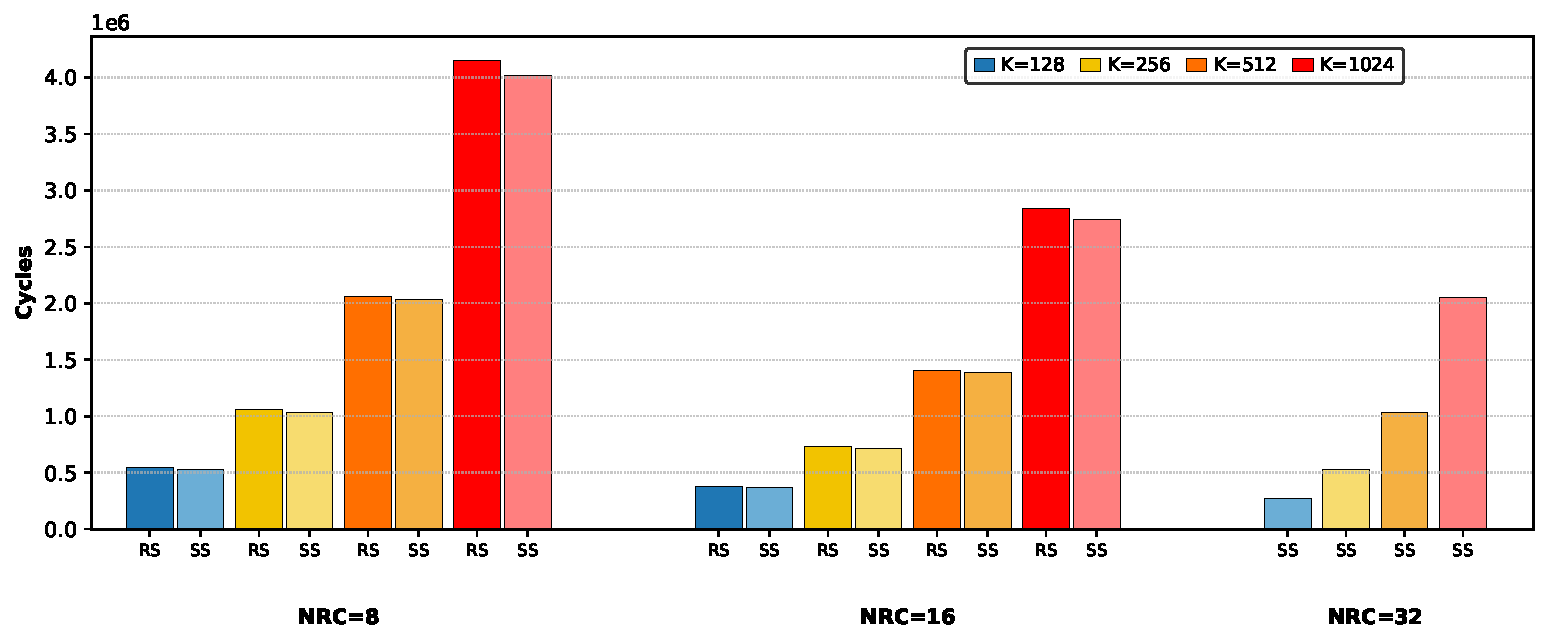
\includegraphics[width=\linewidth]
    {hpca2027-latex-template/fig/nrc_sweep_cycles_tintmode_hpca_no_mode_legend_v7.pdf}
    \caption{WGMMA execution cycles as the number of accumulator
    registers is increased in RS and SS modes.}
    \label{fig:nrc_sweep}
\end{figure}

\subsubsection{K vs.\ 2K-Wide FEDP}
Fig.~\ref{fig:fedp2k_sweep} shows that the 2K-wide FEDP is able to reduce instruction count by 31--33\% and execution cycles by 28--30\% in both
operand-staging modes. Our evaluations also show that increasing FEDP pipeline latency from four to eight
cycles add less than 2\% overhead. Halving the number of $K$-dimension
micro-ops therefore considerably outweighs the deeper pipeline and extra descriptor-setup micro-op cost.
% REVIEW(2026-10-01): the next sentence moved here from the design section (a measurement); its source run is not identified in the pinned branch d6426cca1 -- coauthors confirm.
The setup micro-op that dense RS mode adds with the 2K-wide FEDP increases the end-to-end cycle count by under 1\%.
\begin{figure}
    \centering
    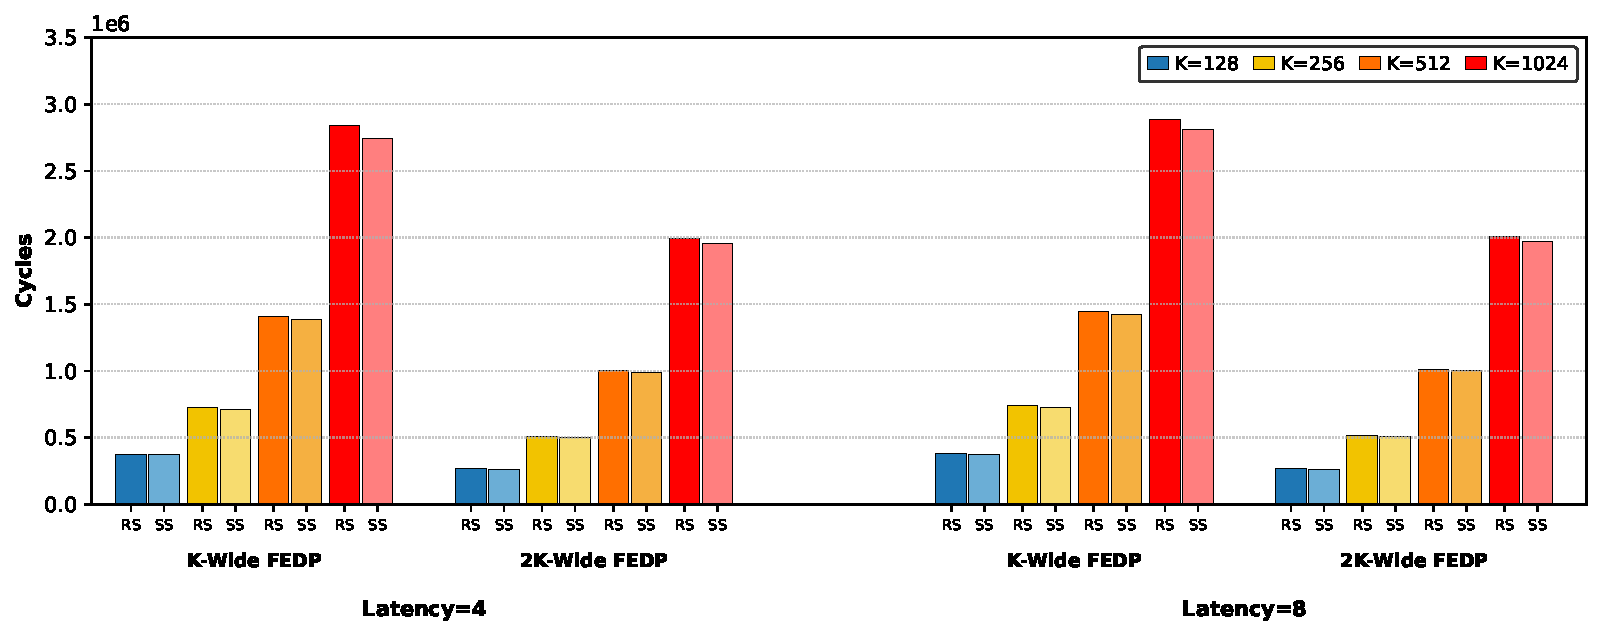
\includegraphics[width=\linewidth]
    {hpca2027-latex-template/fig/fedp2k_cycles_clustered_hpca_ylim35_v4.pdf}
    \caption{WGMMA execution cycles with $K$-wide and $2K$-wide FEDP
    units at four- and eight-cycle pipeline latencies.}
    \label{fig:fedp2k_sweep}
\end{figure}

\subsubsection{TCU SRAM vs.\ Register File WGMMA Descriptor Load}
Moving the WGMMA descriptors into TCU SRAM increases cycles by
1.2--6.5\% relative to register-file delivery. The penalty is largest for short SS kernels
and decreases as more computation amortizes descriptor setup. Relieving
the pressure of two register operands does not offset the added
shared-memory store, synchronization, and AGU traffic. Small control
metadata should therefore remain in the register file unless those
registers enable a larger accumulator configuration or there is extreme register pressure.

\subsection{Sparse Tensor Core Design Space Exploration}\label{sec:eval_sparse}

This subsection answers Q1, the internal mechanisms behind tensor-core sparsity (Section~\ref{sec:mot_causes}). The first two parts explore the sparse design space of FourShadow: the symmetric and asymmetric layouts of warp-level MMA, and the two operand-staging modes of warp-group MMA. The last two parts give the answers by comparing warp-level MMA with 2:4 sparsity on FourShadow and on an NVIDIA RTX 5080 (Sections~\ref{sec:eval_sparse_halves} and~\ref{sec:eval_sparse_meta}, configuration in Section~\ref{sec:methodology}).

\subsubsection{Symmetric vs.\ Asymmetric Sparse Configurations}
Sparsity speeds up the asymmetric layouts in every cell of
Fig.~\ref{fig:sparse_sym_sweep} and the symmetric layouts less. The 8- and
32-thread cells span 1.24--1.78$\times$, with the maximum for TF32 at
$K{=}1024$ and 8 threads, and both symmetric cells sit below both
asymmetric cells in 11 of 12 rows (the exception: TF32 at $K{=}256$,
1.45$\times$ at 16 threads against 1.37$\times$ at 8). At 4 threads
sparsity loses in nine of 12 cells (0.71--0.83$\times$); at 16 threads
it gains modestly, 0.91--1.45$\times$ and above 1 in 11 of 12 cells. The
ordering follows Section~\ref{sec:design_sparse}: only the asymmetric
layouts halve the micro-ops of a sparse WMMA. The symmetric layouts keep
the dense micro-op count, which therefore explains neither the 4-thread
loss nor the 16-thread gain; their source is not isolated.
\begin{figure}[t]
    \centering
    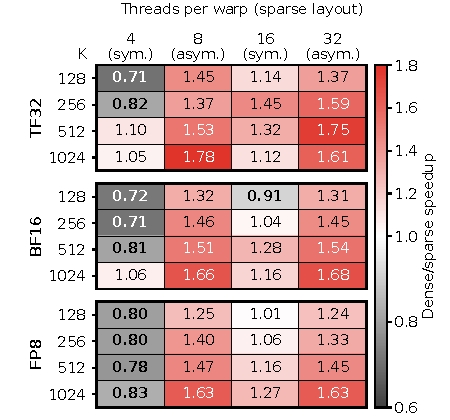
\includegraphics[width=0.9\linewidth]
    {hpca2027-latex-template/fig/sparse_sym_asym_iw1_nw4.pdf}
    \caption{Dense-over-sparse speedup of a $128{\times}128{\times}K$ GEMM
    with warp-level MMA at (IW-1, NW-4), from total kernel cycles on SimX.
    Each cell prints the speedup; cells below 1 (sparse slower than dense)
    are grey with bold values.}
    \label{fig:sparse_sym_sweep}
\end{figure}

\subsubsection{Dense vs.\ Sparse in RS and SS Modes}
\begin{figure}[t]
    \centering
    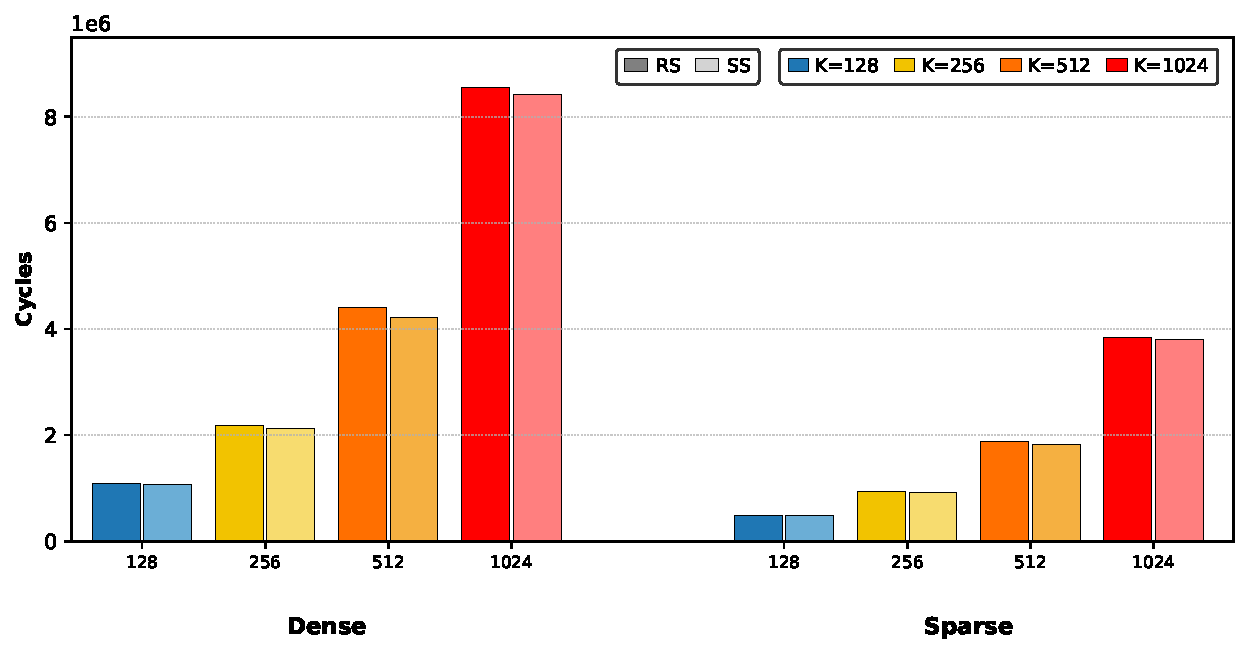
\includegraphics[width=\linewidth]
    {hpca2027-latex-template/fig/sparse_wg_cycles_clustered_newdata_v3.pdf}
    \caption{Dense and 2:4 sparse BF16 WGMMA execution cycles in
    RS and SS operand-staging modes.}
    \label{fig:sparse_wg_sweep}
\end{figure}

% REVIEW(2026-10-01): configuration behind these numbers not yet reconciled with Sec. C.3 (max 1.78x whole-processor, 1.75x in-kernel region, measured for warp-level MMA + SP); see rebuttal_plan.md
Fig.~\ref{fig:sparse_wg_sweep} shows that sparsity reduces cycles by
54.8--57.4\% in RS mode and 54.9--56.9\% in SS mode, corresponding to
2.21--2.35$\times$ speedup. Agreeing with the sparse wargroup MMA microbenchmarking in \cite{luo2025dissectingnvidiahopperarchitecture}, this is the only case where RS mode is faster than or equal to SS mode. 

\subsubsection{Only Part of the Sparse Cost Halves}\label{sec:eval_sparse_halves}
\begin{figure*}[t]
    \centering
    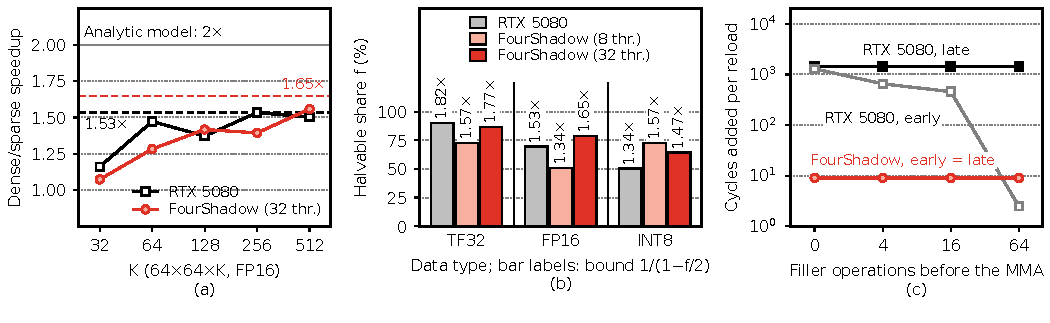
\includegraphics[width=\textwidth]
    {hpca2027-latex-template/fig/paper_sparse_nvidia_compare.pdf}
    \caption{Warp-level MMA with 2:4 sparsity on FourShadow and on an
    NVIDIA RTX 5080, both timed over the in-kernel region.
    (a)~Dense-over-sparse speedup of a $64{\times}64{\times}K$ FP16 GEMM;
    each dashed line is the bound $1/(1-f/2)$ of the platform of the same colour.
    (b)~Halvable share $f$ of the per-$K$ cost per data type, from the
    $64{\times}64{\times}K$ fits (INT8 fits use $K\geq64$); the bar labels give
    the bound.
    (c)~Cycles that one metadata reload adds per iteration against the number
    of filler operations before the sparse MMA, FP16, on a logarithmic axis:
    one warp of the RTX 5080; FourShadow at (IW-1, NW-4) with one warp alone,
    where the early and late schedules coincide, and with four one-warp CTAs
    on the issue lane at 32 threads per warp (cycles per CTA).}
    \label{fig:sparse_nvidia}
\end{figure*}

For the $64{\times}64{\times}K$ FP16 GEMM of Fig.~\ref{fig:sparse_nvidia}(a), the dense-over-sparse speedup rises from 1.16$\times$ at $K{=}32$ to 1.50$\times$ at $K{=}512$ on the RTX 5080, and from 1.07$\times$ to 1.56$\times$ on FourShadow at 32 threads per warp. Sparsity is faster in each of the 17 shapes measured on both platforms, and the two speedups differ by a median of 6.2\% at 32 threads and 9.0\% at 8 threads; at $128{\times}128{\times}1024$ they diverge, which we leave unexplained (1.40$\times$ on the RTX 5080 against 1.51$\times$ and 1.65$\times$ on FourShadow at 8 and 32 threads). Over issue widths of 1, 2 and 4 with 4 or 16 warps, at 8 and 32 threads, FourShadow stays below 2$\times$: its maximum is 1.92$\times$, for the INT8 $128{\times}128{\times}1024$ GEMM at (IW-1, NW-16) and 32 threads.

We fit the cycles of each $K$ sweep as $C_{\mathrm{dense}} = c + (a+d)K$ and $C_{\mathrm{sparse}} = c' + (a/2+d)K$, where $a$ is the per-$K$ cost that 2:4 sparsity halves and $d$ the per-$K$ cost that it leaves unchanged ($c$ and $c'$ do not depend on $K$); as $K$ grows the speedup approaches $1/(1-f/2)$, where $f = a/(a+d)$ is the halvable share. For FP16, $f$ is 69.7\% on the RTX 5080 and 78.5\% on FourShadow at 32 threads, which gives the dashed lines of Fig.~\ref{fig:sparse_nvidia}(a) at 1.53$\times$ and 1.65$\times$. In Fig.~\ref{fig:sparse_analytic}, $a$ contains $\mathit{TC}$ and the $A$ load, which halve together, and $d$ the $B$ load and the metadata.

On the RTX 5080 the halvable share falls as the data type narrows, from 90.1\% for TF32 to 50.5\% for INT8 (grey bars of Fig.~\ref{fig:sparse_nvidia}(b)), which lowers the bound from 1.82$\times$ to 1.34$\times$, and one sparse MMA instruction, which covers twice the $K$ of a dense one, costs 1.10, 1.30 and 1.50 times its cycles for TF32, FP16 and INT8. FourShadow shows the order at 32 threads (86.9\%, 78.5\% and 64.4\%) and not at 8 threads (72.9\%, 50.7\% and 72.9\%), so the precision dependence is a property of the RTX 5080, not an agreement between the platforms. We state two candidate mechanisms as hypotheses. First, loads overlap with compute, so an MMA step costs about the longer of the two: on the RTX 5080 the halvable cost of a dense step falls from 5.11 cycles per output element for TF32 to 1.94 for INT8 while the cost that does not halve rises from 0.56 to 1.91. Second, the selection of operands by the metadata widens with the elements per instruction, 64 positions of $K$ for a sparse INT8 instruction against 16 for TF32.

\answerbox{Answer \#1 for Q1}{2:4 sparsity halves only part of the per-$K$ cost of a tensor-core GEMM, so its speedup stays below 2$\times$ and depends on the size of that halvable part, which changes with precision: on the RTX 5080 it shrinks as the data type narrows, and the bound falls from 1.82$\times$ for TF32 to 1.34$\times$ for INT8.}

\subsubsection{One RTX 5080 Warp Hides Its Metadata Load; FourShadow Needs Several}\label{sec:eval_sparse_meta}
On the RTX 5080, one CTA of one warp reloads the metadata, an ordinary register operand of \texttt{mma.sp}, in each of 256 iterations of a sparse FP16 MMA, before (early) or after (late) 0 to 64 filler operations (Fig.~\ref{fig:sparse_nvidia}(c)). The late reload adds 363.1 to 364.2 cycles per iteration at every filler distance; the early reload adds 326.2 cycles with no filler and 0.3 cycles with 64 filler operations. An early load thus costs the maximum of the load and the filler, and a late load their sum: the two rules, without a fitted constant, reproduce the cycles within 0.13\% for FP16 and within 0.72\% over six data formats. With 16 filler operations the profiled long-scoreboard stall share is 26.8\% early and 55.2\% late, at the same 11,858 instructions and 269 load requests.

On FourShadow at (IW-1, NW-4), a dedicated instruction loads the metadata into a per-warp memory (Section~\ref{sec:design_sparse}), and with one CTA of one active warp the reload adds 9.0 cycles per iteration, early or late, at 8 and 32 threads per warp. When four one-warp CTAs share the issue lane at 32 threads per warp, the reload adds 59.3 cycles per CTA with no filler, and from 4 to 64 filler operations the late reload stays between 58.0 and 62.1 cycles while the early reload falls from 28.7 to 7.6 cycles (sum and maximum rules within 1.7\% and 4.6\%). This separation is stated for 32 threads only, because at 8 threads the late reload also falls, from 51.9 to 11.6 cycles; the scope is a simulation of one-warp CTAs on a lane of four warp slots, and absolute cycles are not compared across the platforms.

\answerbox{Answer \#2 for Q1}{The cost of sparse metadata depends on where the kernel issues the load and on what can run while it is pending: one RTX 5080 warp hides an early load behind its own work, whereas FourShadow at (IW-1, NW-4) and 32 threads per warp hides it only behind other warps.}

\subsection{FPGA Design Flow}

We implement FourShadow on an AMD Alveo U55C with 16\,GB HBM2 and
target a 250\,MHz clock frequency. The evaluated system contains
one core with eight 8-thread warps, an issue width of four, and four
8-lane Ten-Four\cite{rout2026tenfouropensourcefuseddot} blocks supporting FP16 inputs and FP32
accumulation, WGMMA, 2K-wide FEDP, and 2:4 structured sparsity. Table.~\ref{tab:tcu-parts} shows the hierarchial utilization overhead of each FourShadow extended unit.
Of the post-synthesis LUT area of the fully enabled Vortex core, the TCU
takes 53.7\%, the issue stage and front end 17.2\%, the FPU 13.8\%, the ALU
6.1\%, memory (first-level caches and local memory) 4.8\%, the LSU 2.1\%,
the SFU 1.6\% and the remainder 0.7\%.

\begin{table}
  \centering
  \caption{Post-synthesis resource breakdown of the fully enabled
  FourShadow TCU.}
  \label{tab:tcu-parts}
  \setlength{\tabcolsep}{5pt}
  \renewcommand{\arraystretch}{1.15}
  \begin{tabular}{@{}lrrrr@{}}
  \toprule
  \textbf{Part} & \textbf{LUT} & \textbf{FF} &
  \textbf{BRAM} & \textbf{DSP} \\
  \midrule
  FEDP array ($4\times$)             & 47\,533 & 14\,800 & 0  & 128 \\
  Lane dispatch                      & 18\,665 & 6\,990  & 0  & 0   \\
  WGMMA control                      & 17\,183 & 5\,149  & 0  & 2   \\
  A operand buffers ($4\times$)      & 16\,476 & 4\,493  & 0  & 0   \\
  Lane gather                        & 1\,638  & 2\,240  & 0  & 0   \\
  AGU                                & 1\,490  & 1\,303  & 0  & 0   \\
  2:4 sparsity metadata SRAM         & 1\,056  & 0       & 32 & 0   \\
  B buffer, FIFOs, and glue          & 772     & 64      & 4  & 0   \\
  \midrule
  \textbf{TCU total}                 &
  \textbf{104\,813} & \textbf{35\,039} &
  \textbf{36} & \textbf{130} \\
  \bottomrule
  \end{tabular}
\end{table}

Fig.~\ref{fig:e2e_fpga} shows that WGMMA provides its largest gains
when matrix operations dominate execution. It raises NeRF from
4.72$\times$ to 26.17$\times$, Llama~2 prefill from 5.91$\times$ to
9.15$\times$, and decode from 1.42$\times$ to 2.00$\times$, while CNN,
attention, and FlashAttention remain nearly unchanged. Sparsity alone
benefits NeRF and slightly improves attention, but its metadata and
compression overhead reduce performance for CNN and both Llama~2
phases. Combining sparsity with WGMMA reaches 16.88$\times$ for CNN
and 26.82$\times$ for NeRF, showing that the two extensions are
workload-dependent rather than uniformly additive.
\begin{figure}
    \centering
    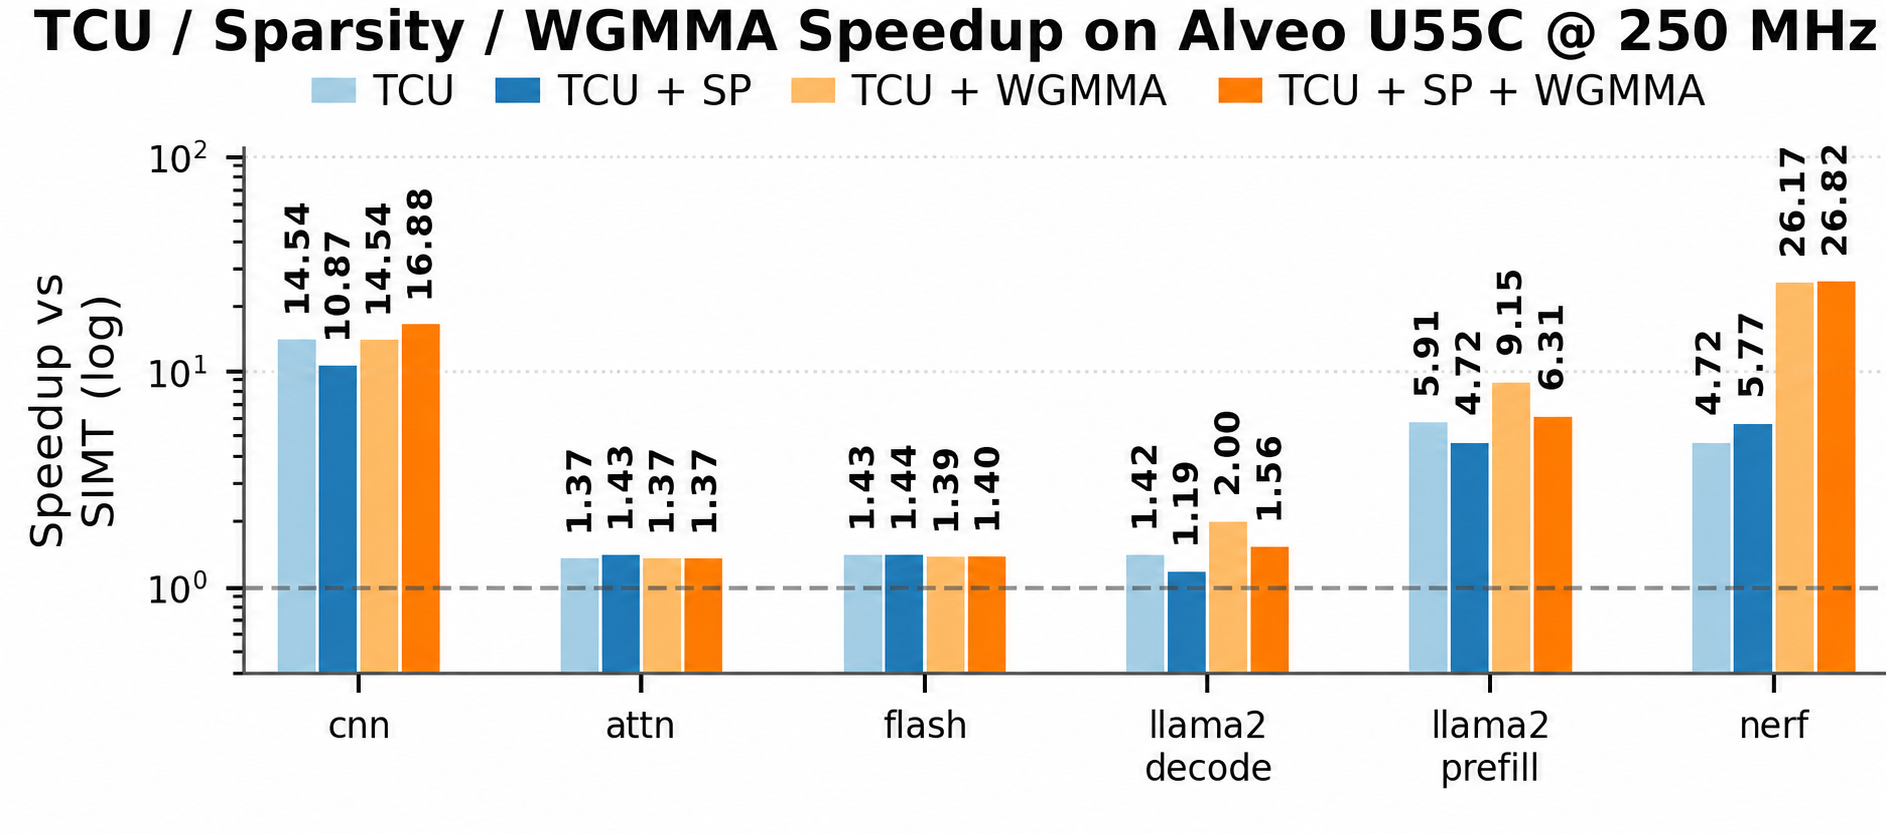
\includegraphics[width=\linewidth]
    {hpca2027-latex-template/fig/fpga_e2e.png}
    \caption{End-to-end FPGA speedup over the SIMT baseline on the
    Alveo U55C at 250\,MHz.}
    \label{fig:e2e_fpga}
\end{figure}

\subsection{ASIC Design Flow}

\subsubsection{ASIC Synthesis and Timing}

We synthesize the standalone FourShadow TCU using Synopsys Design
Compiler X-2025.06-SP1 with the ASAP7 7\,nm
\texttt{asap7sc7p5t\_28} NLDM TT predictive PDK library.

\subsubsection{Threads/Warp Area--Performance Tradeoff}
Fig.~\ref{fig:pareto} combines synthesized TCU area with end-to-end application evaluation performance. Llama~2 prefill reaches 12.7$\times$ at $NT{=}16$
and then slightly regresses at $NT{=}32$, despite the TCU area more
than doubling. Decode shows a stronger optimum, rising to
6.2$\times$ at $NT{=}16$ before falling to approximately 3$\times$
at $NT{=}32$. NeRF instead continues to benefit from wider warps and
reaches its highest speedup at $NT{=}32$. The preferred warp width is
therefore workload-dependent, although $NT{=}16$ consistently provides the best
area--performance ratio for both Llama~2 phases.
\begin{figure}
    \centering
    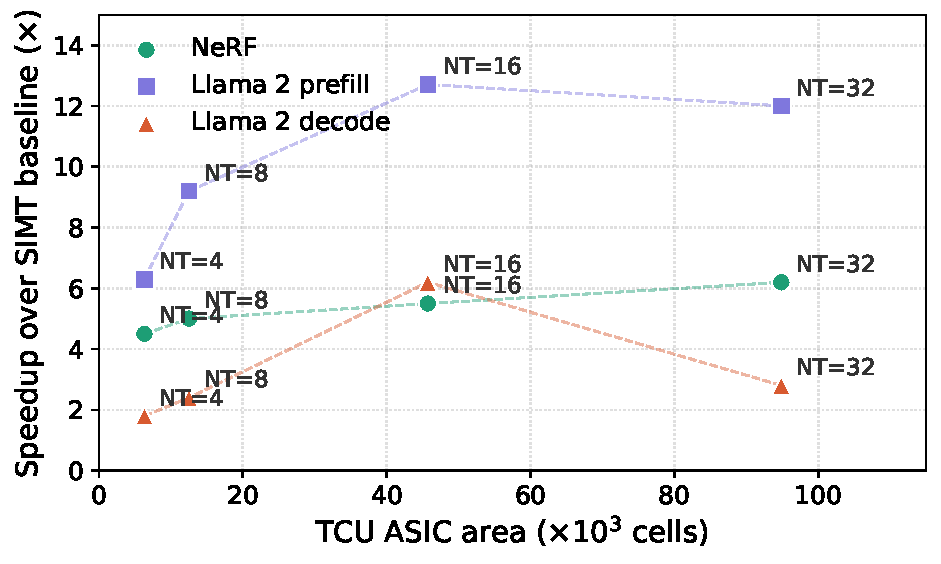
\includegraphics[width=0.9\linewidth]
    {hpca2027-latex-template/fig/pareto.pdf}
    \caption{End-to-end SimX speedup over the SIMT baseline versus
    synthesized TCU cell area across threads/warp configurations.}
    \label{fig:pareto}
\end{figure}

\subsubsection{Issue-Width Area--Performance Tradeoff}
Fig.~\ref{fig:iw_area_scaling} shows that TCU area scales almost
linearly with issue width, increasing from 58.6\,k$\mu$m$^2$ at
$IW{=}1$ to 115.6 and 230.6\,k$\mu$m$^2$ at $IW{=}2$ and $IW{=}4$.
However, performance scales much more slowly, reaching 1.37--1.41$\times$ at
$IW{=}2$ and 1.66--1.70$\times$ at $IW{=}4$. Doubling the area again
to an estimated 455--462\,k$\mu$m$^2$ at $IW{=}8$ raises speedup to
only 1.70--1.81$\times$. Thus, $IW{=}4$ forms the practical optimal on the curve, beyond which additional TCU blocks and larger warp-groups are increasingly
limited by operand delivery and non-TCU execution rather than
arithmetic capacity.
\begin{figure}
    \centering
    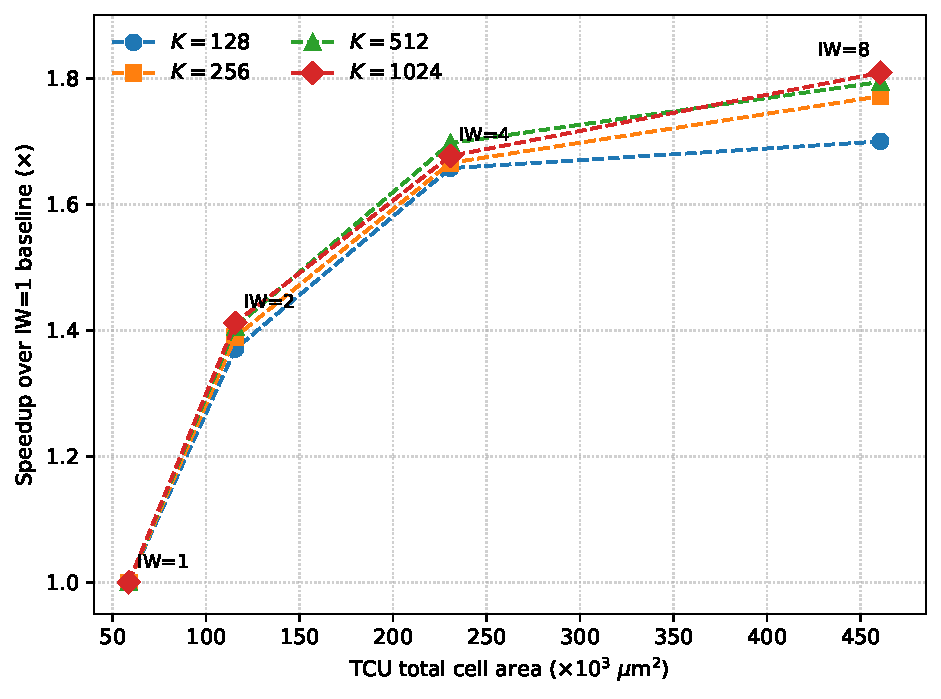
\includegraphics[width=0.9\linewidth]
    {hpca2027-latex-template/fig/iw_scaling_area_speedup_nt16.pdf}
    \caption{WGMMA speedup over $IW{=}1$ versus synthesized TCU cell
    area at $NT{=}16$. The $IW{=}8$ area is projected from the
    measured $IW\leq4$ designs.}
    \label{fig:iw_area_scaling}
\end{figure}